%%%%%%%%%%%%%%%%%%%%%%%%%%%%%%%%%%%%%%%%%%%%%%%%%%%%%%%%%%%%%%%%%%%%%%%%%%%%%%%%%%%%%%%%%%%%%%%%%%%%%%%%%%%%%%%%%%%%%%%%%%%%%%%%%%%%%%%%%%%%%%%%%%%%%%%%%%%
% This is just an example/guide for you to refer to when submitting manuscripts to Frontiers, it is not mandatory to use Frontiers .cls files nor frontiers.tex  %
% This will only generate the Manuscript, the final article will be typeset by Frontiers after acceptance.   
%                                              %
%                                                                                                                                                         %
% When submitting your files, remember to upload this *tex file, the pdf generated with it, the *bib file (if bibliography is not within the *tex) and all the figures.
%%%%%%%%%%%%%%%%%%%%%%%%%%%%%%%%%%%%%%%%%%%%%%%%%%%%%%%%%%%%%%%%%%%%%%%%%%%%%%%%%%%%%%%%%%%%%%%%%%%%%%%%%%%%%%%%%%%%%%%%%%%%%%%%%%%%%%%%%%%%%%%%%%%%%%%%%%%

%%% Version 3.4 Generated 2018/06/15 %%%
%%% You will need to have the following packages installed: datetime, fmtcount, etoolbox, fcprefix, which are normally inlcuded in WinEdt. %%%
%%% In http://www.ctan.org/ you can find the packages and how to install them, if necessary. %%%
%%%  NB logo1.jpg is required in the path in order to correctly compile front page header %%%

\documentclass[utf8]{frontiersSCNS} % for Science, Engineering and Humanities and Social Sciences articles
\usepackage{url,hyperref,lineno,listings,microtype,subcaption}
\usepackage[onehalfspacing]{setspace}

% Automatic formatting of SI units
\usepackage[binary-units,separate-uncertainty=true,range-phrase=--]{siunitx}

% Required for 'straight' quotes in code listings
\usepackage[T1]{fontenc}

% Visible TODO notes
\newcommand{\todo}[1]{\textbf{\textsc{\textcolor{red}{(TODO: #1)}}}}

% Configure code listings
\lstset{language=C++,showstringspaces=false,basicstyle=\tiny,upquote=true,identifierstyle=\ttfamily\color{black}}
\lstset{language=Python,showstringspaces=false,basicstyle=\tiny,upquote=true,identifierstyle=\ttfamily\color{black}}

\linenumbers


\def\keyFont{\fontsize{8}{11}\helveticabold }
\def\firstAuthorLast{Knight and Nowotny} %use et al only if is more than 1 author
\def\Authors{James C Knight\,$^{1,*}$, Anton Komissarov\,$^{2}$, Thomas Nowotny\,$^{1}$}
\def\Address{$^{1}$Centre for Computational Neuroscience and Robotics, School of Engineering and Informatics, University of Sussex, Brighton, United Kingdom  \\
$^{2}$\todo{Anton's affiliatino}}
\def\corrAuthor{James C Knight}
\def\corrEmail{J.C.Knight@sussex.ac.uk}

\begin{document}
\onecolumn
\firstpage{1}

\title[PyGeNN]{PyGeNN: A Python library for GPU-enhanced neural networks} 

\author[\firstAuthorLast ]{\Authors} %This field will be automatically populated
\address{} %This field will be automatically populated
\correspondance{} %This field will be automatically populated

\extraAuth{}% If there are more than 1 corresponding author, comment this line and uncomment the next one.
%\extraAuth{corresponding Author2 \\ Laboratory X2, Institute X2, Department X2, Organization X2, Street X2, City X2 , State XX2 (only USA, Canada and Australia), Zip Code2, X2 Country X2, email2@uni2.edu}


\maketitle


\begin{abstract}

%%% Leave the Abstract empty if your article does not require one, please see the Summary Table for full details.
\section{}
For full guidelines regarding your manuscript please refer to \href{http://www.frontiersin.org/about/AuthorGuidelines}{Author Guidelines}.

As a primary goal, the abstract should render the general significance and conceptual advance of the work clearly accessible to a broad readership. References should not be cited in the abstract. Leave the Abstract empty if your article does not require one, please see \href{http://www.frontiersin.org/about/AuthorGuidelines#SummaryTable}{Summary Table} for details according to article type. 

\tiny
 \keyFont{ \section{Keywords:} GPU, high-performance computing,
   parallel computing, benchmarking, computational neuroscience, spiking neural networks, Python} %All article types: you may provide up to 8 keywords; at least 5 are mandatory.
\end{abstract}

\section{Introduction}
A wide range of spiking neural network~(SNN) simulators are available, each with their own application domains. 
NEST~\citep{Gewaltig2007} is widely used for large-scale point neuron simulations on distributed computing systems; NEURON~\citep{carnevale2006neuron} and Arbor~\citep{Akar2019} specialise in the simulation of complex multi-compartmental models; NeuroKernel~\citep{Givon2016} is focused on emulating fly brain circuits using Graphics Processing Units~(GPUs); and CARLsim~\citep{Chou2018}, ANNarchy~\citep{Dinkelbach2015}, NeuronGPU~\citep{Golosio2020} and GeNN~\citep{Yavuz2016} use GPUs to accelerate point neuron models. 
For performance reasons, many of these simulators are written in C++ and, especially amongst the older simulators, users describe their models either using a Domain-Specific Language~(DSL) or directly in C++.
For programming language purists, a DSL may be an elegant way of describing an SNN network model and, for simulator developers, not having to add bindings to another language is convenient.
However, both choices act as a barrier to potential users.
Therefore, with both the computational neuroscience and machine learning communities gradually coalescing towards a Python-based ecosystem with a wealth of mature libraries for scientific computing~\citep{Hunter2007,VanDerWalt2011,Millman2011}, exposing spiking neural network simulators to Python seems a pragmatic choice.
NEST~\citep{Eppler2009}, NEURON~\citep{Hines2009} and CARLsim~\citep{Balaji2020} have all taken this route and now offer a Python interface.
Furthermore, newer simulators such as Arbor and Brian2~\citep{Stimberg2019} have been designed from the ground up with a Python interface.

While we have recently demonstrated some very competitive performance results~\citep{Knight2018,Knight2020} using our GeNN simulator~(Yavuz2016), it has so far not been usable directly from Python.
GeNN can already be used as a backend for the Python-based Brian2 simulator~\citep{Stimberg2019}. In brief, the Brian2GeNN interface~\citep{Stimberg2020} modifies the C++ backend ``cpp\_standalone'' of Brian 2 to generate C++ input files for GeNN. As for cpp\_standalone, initialisation of simulations is mostly done in C++ on the CPU and recording data is saved into binary files and re-imported into Python using Brian 2's native methods. While Brian2GeNN allows Brian2 users to harness the performance benefits that GeNN provides, it is not possible to expose all of GeNN's unique features to Python through the Brian2 API.
Specifically, GeNN not only allows users to easily define their own neuron and synapse models but, also `snippets' for offloading the potentially costly initialisation of model parameters and connectivity onto the GPU.
Additionally, GeNN  provides a lot of freedom for users to integrate their own code into the simulation loop.
In this paper we describe the implementation of PyGeNN -- a Python package which aims to expose the full range of GeNN functionality with minimal performance overheads.
While implementing new neuron and synapse models in the majority of other GPU simulators requires extending the underling C++ code, using PyGeNN, models can be defined directly from Python.
Finally, we demonstrate the flexibility and performance of PyGeNN in two scenarios where minimising performance overheads is particularly critical.
\begin{itemize}
    \item In a simulation of a large, highly-connected model of a cortical microcircuit~\citep{Potjans2012} with small simulation timesteps. Here the cost of copying spike data off the GPU from a large number of neurons every timestep can become a bottleneck.
    \item In a simulation of a much smaller model of Pavlovian conditioning~\citep{Izhikevich2007} where learning occurs over \SI{1}{\hour} of biological time and stimuli are delivered -- following a complex scheme -- throughout the simulation. Here any overheads are multiplied by a large number of timesteps and copying stimuli to the GPU can become a bottleneck.
\end{itemize}
Using the facilities provided by PyGeNN, we show that both scenarios can be simulated from Python with only minimal overheads over a pure C++ implementation.

\section{Materials and Methods}
\subsection{GeNN}
\label{sec:methods/genn}
GeNN~\citep{Yavuz2016} is a library for generating CUDA code for the simulation of spiking neural network models.
GeNN handles much of the complexity of using CUDA directly as well as automatically performing device-specific optimizations so as to to maximize performance.

GeNN consists of a main library -- implementing the API used to define models as well as the generic parts of the code generator -- and an additional library for each backend (currently there is a reference C++ backend for generating CPU code and a CUDA backend. An OpenCL backend is under development).
Users describe their model by implementing a \lstinline{modelDefinition} function within a C++ file. For example, a model consisting of 4 Izhikevich neurons with heterogeneous parameters, driven by a constant input current might be defined as follows:
%
\begin{lstlisting}[language=C++]
void modelDefinition(ModelSpec &model)
{
    model.setDT(0.1);
    model.setName("izhikevich");
    
    NeuronModels::IzhikevichVariable::VarValues popInit(
        -65.0, -20.0, uninitialisedVar(), uninitialisedVar(),
        uninitialisedVar(), uninitialisedVar());
    
    model.addNeuronPopulation<NeuronModels::IzhikevichVariable>(
        "Pop", 4, {}, popInit);

    model.addCurrentSource<CurrentSourceModels::DC>(
        "CS", "Pop", {10.0}, {});
}
\end{lstlisting}
%
The \emph{genn-buildmodel} command line tool is then used to compile this file; link it against the main GeNN library and the desired backend library; and finally run the resultant executable to generate the source code required to build a simulation dynamic library (a .dll file on Windows or a .so file on Linux and Mac).
This dynamic library can then either be statically linked against a simulation loop provided by the user or dynamically loaded by the user's simulation code.
To demonstrate this latter approach, this example uses the \lstinline{SharedLibraryModel} helper class supplied with GeNN to dynamically load the previously defined model, initialise the heterogenous neuron parameters and print each neuron's membrane voltage every timestep: 
%
\begin{lstlisting}[language=C++]
#include "sharedLibraryModel.h"

int main()
{
    SharedLibraryModel<float> model("./", "izhikevich");
    model.allocateMem();
    model.initialize();
    float *aPop = model.getScalar<float>("a");
    float *bPop = model.getScalar<float>("b");
    float *cPop = model.getScalar<float>("c");
    float *dPop = model.getScalar<float>("d");
    aPop[0] = 0.02; bPop[0] = 0.2;  cPop[0] = -65.0;    dPop[0] = 8.0;  // RS
    aPop[1] = 0.1;  bPop[1] = 0.2;  cPop[1] = -65.0;    dPop[1] = 2.0;  // FS
    aPop[2] = 0.02; bPop[2] = 0.2;  cPop[2] = -50.0;    dPop[2] = 2.0;  // CH
    aPop[3] = 0.02; bPop[3] = 0.2;  cPop[3] = -55.0;    dPop[3] = 4.0;  // IB
    model.initializeSparse();

    float *vPop = model.getScalar<float>("VPop");
    while(model.getTime() < 200.0f) {
        model.stepTime();
        model.pullVarFromDevice("Pop", "V");
        printf("%f, %f, %f, %f, %f\n", t, VPop[0], VPop[1], VPop[2], VPop[3]);
    }
    return EXIT_SUCCESS;
}
\end{lstlisting}

\subsection{SWIG}
In order to use GeNN from Python, both the model creation API and the \lstinline{SharedLibraryModel} functionality need to be `wrapped' so they can be called from Python.
While this is possible using the API built into Python itself, a wrapper function would need to be manually implemented for each GeNN function to be exposed which would result in a lot of maintenance overhead.
Instead, we chose to use SWIG~\citep{Beazley1996} to automatically generate wrapper functions and classes. 
SWIG generates Python modules based on special interface files which can directly include C++ code as well as special `directives' which control SWIG, for instance:
%
\begin{lstlisting}[language=C++]
%module(package="package") package
%include "test.h" 
\end{lstlisting}
%
where the \lstinline{%module} directive sets the name of the generated module and the package it will be located in and the \lstinline{%include} directive parses and automatically generates wrapper functions for a C++ header file.
We use SWIG in this manner to wrap both the model building and \lstinline{SharedLibraryModel} APIs described in section~\ref{sec:methods/genn}.
However, key parts of GeNN's API such as the \lstinline{ModelSpec::addNeuronPopulation} method employed in section~\ref{sec:methods/genn}, rely on C++ templates which are not directly translatable to Python.
Instead, valid template instantiations need to be given a unique name in Python using the \lstinline{%template} SWIG directive:
%
\begin{lstlisting}[language=C++]
%template(addNeuronPopulationLIF) ModelSpec::addNeuronPopulation<NeuronModels::LIF>;
\end{lstlisting}
%
Having to manually add these directives whenever a model is added to GeNN would be exactly the sort of maintenance overhead we were trying to avoid by using SWIG.
Instead, when building the Python wrapper, we search the GeNN header files for the macros used to declare models in C++ and automatically generate SWIG \lstinline{%template} directives.

As previously discussed, a key feature of GeNN is the ease with which it allows users to define their own neuron and synapse models as well as `snippets' defining how variables and connectivity should be initialised.
Beneath the syntactic sugar described in our previous work~\citep{Knight2018}, new models can be defined in C++ by defining a new class derived from, for example, the \lstinline{NeuronModels::Base} class.
The ability to extend this system to Python was a key requirement of PyGeNN and, by using SWIG `directors', C++ classes can be made inheritable from Python using a single SWIG directive:
%
\begin{lstlisting}[language=C++]
%feature("director") NeuronModels::Base; 
\end{lstlisting}

\subsection{PyGeNN}
\label{sec:methods/pygenn}
While GeNN \emph{could} be used from Python via the wrapper generated using the techniques described in the previous section, the resultant code would be unpleasant to use directly.
For example, rather than being able to specify neuron parameters using a native Python data structure such as a list or dictionary, one would have to use a wrapped type such as \lstinline{DoubleVector([0.25, 10.0, 0.0, 0.0, 20.0, 2.0, 0.5])}.
To provide a more user-friendly and pythonic interface, we have built PyGeNN on top of the wrapper generated by SWIG.
PyGeNN combines the separate model building and simulation stages of building a GeNN model in C++ into a single API, likely to be more familiar to users of existing Python-based model description languages such as PyNEST~\citep{Eppler2009} or PyNN~\citep{Davison2008}.
By combining the two stages together, PyGeNN can provide a unified dictionary-based API for initialising homogeneous and heterogeneous parameters as shown in this re-implementation of the previous example:
%
\begin{lstlisting}[language=Python]
from pygenn import genn_wrapper, genn_model

model = genn_model.GeNNModel("float", "izhikevich")
model.dT = 0.1

izk_init = {"V": -65.0,
            "U": -20.0,
            "a": [0.02,     0.1,    0.02,   0.02],
            "b": [0.2,      0.2,    0.2,    0.2],
            "c": [-65.0,    -65.0,  -50.0,  -55.0],
            "d": [8.0,      2.0,    2.0,    4.0]}

pop = model.add_neuron_population("Pop", 4, "IzhikevichVariable", {}, izk_init)
model.add_current_source("CS", "DC", "Pop", {"amp": 10.0}, {})

model.build()
model.load()

v = pop.vars["V"].view
while model.t < 200.0:
    model.step_time()
    model.pull_state_from_device("Pop")
    print("%t, %f, %f, %f, %f" % (model.t, v[0], v[1], v[2], v[3]))
\end{lstlisting}
%
Initialisation of variables with homogeneous values -- such as the neurons' membrane potential -- is performed by GeNN and those with heterogeneous values -- such as the \lstinline{a}, \lstinline{b} and \lstinline{c} parameters -- are initialised by PyGeNN when the model is loaded.
While the PyGeNN API is more pythonic and, hopefully, more user-friendly than the C++ interface, it still provides users with the same low-level control over the simulation.
Furthermore, by using SWIG's numpy~\citep{VanDerWalt2011} interface, the host memory allocated by GeNN can be accessed directly from Python using the \lstinline{pop.vars["V"].view} syntax meaning that no potentially expensive additional copying of data is required.

As illustrated in the previously-defined model, for convenience, PyGeNN allows users to access GeNN's built-in models.
However, one of PyGeNN's most powerful features is that it enables users to easily define their own neuron and synapse models from within Python.
For example, an Izhikevich neuron model~\citep{Izhikevich2003a} can be defined using the \lstinline{create_custom_neuron_class} helper function which provides some syntactic sugar over the model class inheritance described in the previous section:
%
\begin{lstlisting}[language=Python]
izk_model = genn_model.create_custom_neuron_class(
    "izk",

    param_names=["a", "b", "c", "d"],
    var_name_types=[("V", "scalar"), ("U", "scalar")],

    sim_code=
        """
        $(V)+=0.5*(0.04*$(V)*$(V)+5.0*$(V)+140.0-$(U)+$(Isyn))*DT;
        $(V)+=0.5*(0.04*$(V)*$(V)+5.0*$(V)+140.0-$(U)+$(Isyn))*DT;
        $(U)+=$(a)*($(b)*$(V)-$(U))*DT;
        """,
    threshold_condition_code="$(V) >= 30.0",
    reset_code=
        """
        $(V)=$(c);
        $(U)+=$(d);
        """)
\end{lstlisting}
%
The \lstinline{param_names} list defines the real-valued parameters that are constant across the whole population of neurons and the \lstinline{var_name_types} list defines the model state variables and their type (the \lstinline{scalar} type is an alias for single or double-precision floating point, depending on the precision passed to the \lstinline{GeNNModel} constructor).
The behaviour of the model can then be defined using a number of code strings.
Unlike in tools like Brian 2~\citep{Stimberg2019}, these code strings are specified in a C-like language rather than in terms of differential equations.
This allows expert users to choose their own solver for models described in terms of differential equations and to programatically define models such as spike sources.
For example, in our example model, we chose to implement this neuron using the idiomatic forward Euler integration scheme employed by \citet{Izhikevich2003a}.
Finally, the \lstinline{threshold_condition_code} expression defines \emph{when} the neuron will spike whereas the \lstinline{reset_code} code string defines how the state variables should be reset after a spike.
%
\begin{figure}[t!]
    \begin{center}
        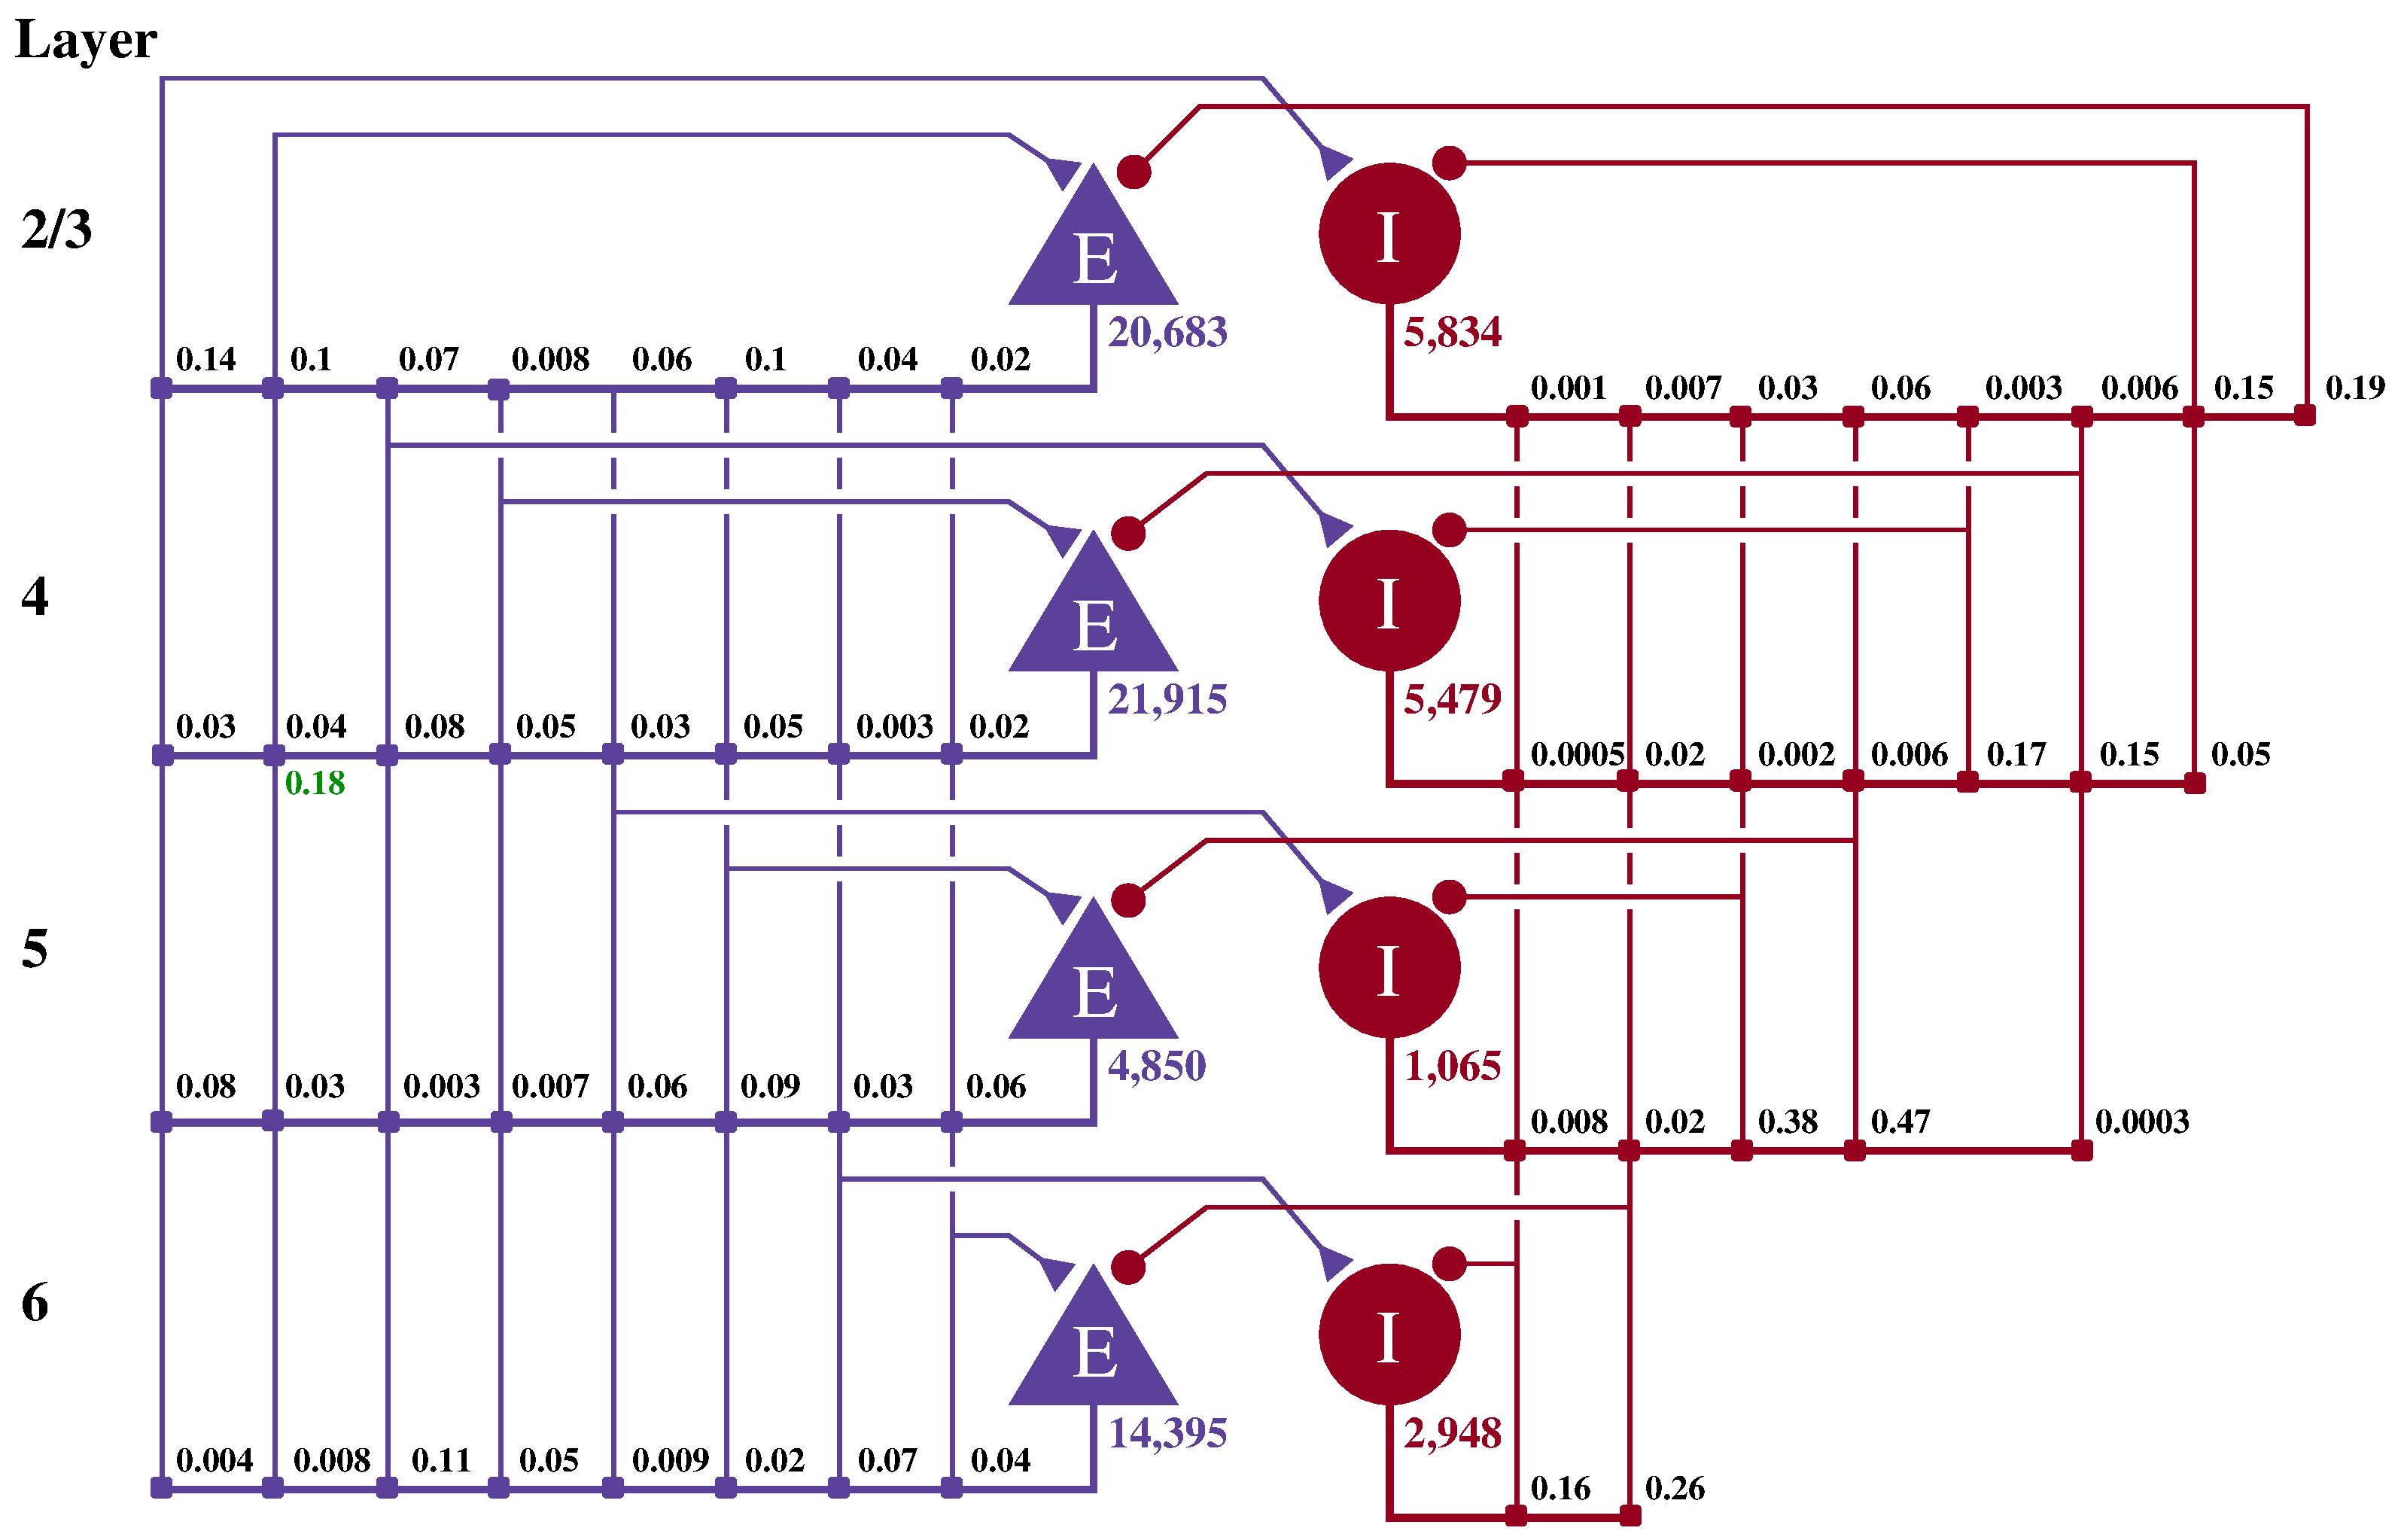
\includegraphics[width=180mm]{figures/potjans_circuit_v2}
    \end{center}
    \caption{Illustration of the microcircuit model.
    Blue triangles represent excitatory populations, red circles represent inhibitory populations and the numbers beneath each symbol shows the number of neurons in each population.
    Connection probabilities are shown in small bold numbers at the appropriate point in the connection matrix.
    All excitatory synaptic weights are normally distributed with a mean of \SI{0.0878}{\nano\ampere} (unless otherwise indicated in green) and a standard deviation of \SI{0.00878}{\nano\ampere}.
    All inhibitory synaptic weights are normally distributed with a mean of \SI{0.3512}{\nano\ampere} and a standard deviation of \SI{0.03512}{\nano\ampere}.}
    \label{fig:potjans_circuit}
\end{figure}
%
\subsection{Spike recording system}
\label{sec:methods/spike_recording}
Internally, GeNN stores the spikes emitted by a neuron population during one simulation timestep in an array containing the indices of the neurons that spiked alongside a counter of how many spikes have been emitted.
Previously, recording spikes in GeNN was very similar to the recording of voltages shown in the previous example code -- the array of neuron indices was simply copied from the GPU to the CPU every timestep.
However, especially when simulating models with a small simulation timestep, such frequent synchronization between the CPU and GPU is costly -- especially if a higher-level language such as Python is involved.
Furthermore, biological neurons typically spike at a low rate (in the cortex, the average firing rate is only around \SI{3}{\hertz}~\citep{Buzsaki2014}) meaning that the amount of spike data transferred every timestep is typically very small.
To address both of these sources of inefficiency, we have added a new data structure to GeNN which stores spike data for many timesteps on device.
To reduce the memory required for this data structure and to make its size independent of neural activity, the spikes emitted by a population of $N$ neurons in a single simulation timestep are stored in a $N\si{\bit}$ bitfield where a `1' represents a spike and a `0' the absence of one.
Spiking data over multiple timesteps is then represented by bitfields stored in a circular buffer.
Using this approach, even the spiking output of relatively large models, running for many timesteps can be stored in a small amount of memory.
For example, the spiking output of a model with \num{100E3} neurons running for \num{10E3} simulation timesteps, required less than \SI{120}{\mega\byte} -- a small fraction of the memory on a modern GPU.
While efficiently handling spikes stored in a bitfield is a little trickier than working with a list of neuron indices, GeNN provides an efficient C++ helper function for saving the spikes stored in a bitfield to a text file and a numpy-based method for decoding them in PyGeNN. 

\subsection{Cortical microcircuit model}
\label{sec:methods/cortical_microcircuit}
\citet{Potjans2012} developed a cortical microcircuit model of \SI{1}{\milli\metre\cubed} of early-sensory cortex.
The model consists of \num{77169} LIF neurons, divided into separate populations representing the excitatory and inhibitory population in each of 4 cortical layers~(2/3, 4, 5 and 6) as illustrated by figure~\ref{fig:potjans_circuit}.
The membrane voltage $V_{i}$ of each neuron $i$ is modelled as
%
\begin{align}
    \tau_{\text{m}} \frac{dV_{i}}{dt} = & (V_{\text{rest}} - V_{i}) + R_{\text{m}}(I_{\text{syn}_{i}} + I_{\text{ext}_{i}}), \label{eq:lif_neuron}
\end{align}
%
where $\tau_{\text{m}} = \SI{10}{\milli\second}$ and $R_{\text{m}} = \SI{40}{\mega\ohm}$ represent the time constant and resistance of the neuron's cell membrane, $V_{\text{rest}} = \SI{-65}{\milli\volt}$ defines the resting potential, $I_{\text{syn}_{i}}$ represents the synaptic input current and $I_{\text{ext}_i}$ represents an external input current.
When the membrane voltage crosses a threshold~$V_{\text{th}} = \SI{-50}{\milli\volt}$ a spike is emitted, the membrane voltage is reset to $V_{\text{rest}}$ and updating of $V$ is suspended for a refractory period $\tau_{\text{ref}} = \SI{2}{\milli\second}$.
Neurons in each population are connected randomly with numbers of synapses derived from an extensive review of the anatomical literature.
These synapses are current-based, i.e.~presynaptic spikes lead to exponentially-decaying input currents $I_{\text{syn}_{i}}$
%
\begin{align}
    \tau_{\text{syn}} \frac{dI_{\text{syn}_{i}}}{dt} = & -I_{\text{syn}_{i}} + \sum_{i=0}^{n} w_{ij} \sum_{t_{j}}  \delta(t - t_{j}),\label{eq:exp_neuron_input_current}
\end{align}
%
where $\tau_{\text{syn}} = \SI{0.5}{\milli\second}$ represents the synaptic time constant and $t_{j}$ are the arrival times of incoming spikes from $n$ presynaptic neurons.
Within each synaptic projection, all synaptic strengths and transmission delays are normally distributed using the parameters presented in \citet[table 5]{Potjans2012} and, in total, the model has approximately \num{0.3E9} synapses.
As well as receiving synaptic input, each neuron in the network also receives an independent Poisson input current, representing input from neighbouring not explicitly modelled cortical regions.
The Poisson input is delivered to each neuron via $I_{\text{ext}_{i}}$ with
%
\begin{align}
    \tau_{\text{syn}} \frac{dI_{\text{ext}_{i}}}{dt} = & -I_{\text{ext}_{i}} + J \text{Poisson}(\nu_{\text{ext}} \Delta t),\label{eq:poisson_input_current}
\end{align}
%
where $\tau_{\text{syn}}=\SI{0.5}{\milli\second}$, $\nu_{\text{ext}}$ represents the mean input rate and $J$ represents the weight.
The ordinary differential equations~\ref{eq:lif_neuron},~\ref{eq:exp_neuron_input_current}~and~\ref{eq:poisson_input_current} are solved with an exponential Euler algorithm.
For a full description of the model parameters, please refer to \citet[tables 4 and 5]{Potjans2012} and for a description of the strategies used by GeNN to parallelise the initialisation and subsequent simulation of this network, please refer to \citet[section 2.3]{Knight2018}.
This model requires simulation using a relatively small timestep of \SI{0.1}{\milli\second}, making the overheads of copying spikes from the GPU every timestep particularly problematic.
%
\begin{figure}[t!]
    \begin{center}
        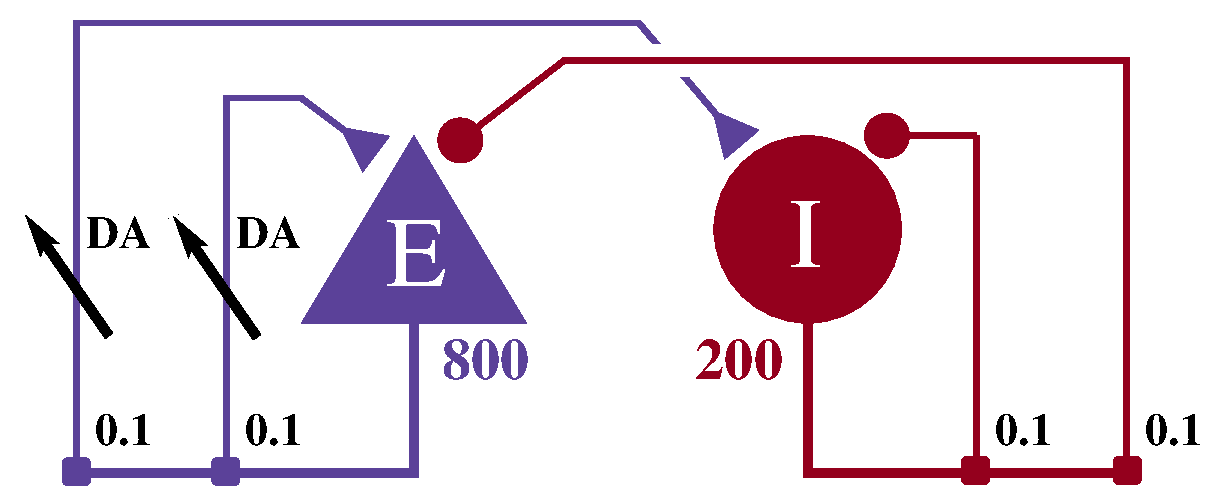
\includegraphics[width=85mm]{figures/circuit2}
    \end{center}
    \caption{Illustration of the balanced random network model.
    The blue triangle represents the excitatory population, the red circle represents the inhibitory population, and the numbers beneath each symbol show the number of neurons in each population.
    Connection probabilities are shown in small bold numbers at the appropriate point in the connection matrix.
    All excitatory synaptic weights are plastic and initialised to \num{1} and all inhibitory synaptic weights are initialised to \num{-1}.}
    \label{fig:potjans_circuit}
\end{figure}
%
\subsection{Pavlovian conditioning model}
\label{sec:methods/izhikevich}
The cortical microcircuit model described in the previous section is ideal for exploring the performance of short simulations of relatively large models.
However, the performance of longer simulations of smaller models is equally vital.\todo{determine e.g. percentage models e.g. on OpenSourceBrain which are small}.
Such models can be particularly troublesome for GPU simulation as, not only might they not offer enough parallelism to fully occupy the device but, each timestep can be simulated so quickly that the overheads of launching kernels etc can dominate.
Additional overheads can be incurred when models require injecting external stimuli throughout the simulation.
Longer simulations are particularly useful when exploring synaptic plasticity so, to explore the performance of PyGeNN in this scenario, we simulate a model of Pavlovian conditioning using a three-factor Spike-Timing-Dependent Plasticity~(STDP) learning rule~\citep{Izhikevich2007}.

\subsubsection{Neuron model}
This model consists of an \num{800} neuron excitatory population and a \num{200} neuron inhibitory population, within which, each neuron $i$ is modelled using the Izhikevich model~\citep{Izhikevich2003a} whose dimensionless membrane voltage $V_{i}$ and adaption variables $U_i$ evolve such that:
%
\begin{align}
    \frac{dV_i}{dt} = & 0.04 V_i^2 + 5V_i + 140 - U_i + I_{\text{syn}_{i}} + I_{\text{ext}_{i}} \label{eq:izhikevich_v} \\
    \frac{dU_i}{dt} = & a(b V_i - U_i) \label{eq:izhikevich_u}
\end{align}
%
When the membrane voltage rises above 30, a spike is emitted and $V_i$ is reset to $c$ and $d$ is added to $U_i$.
Excitatory neurons use the regular-spiking parameters~\citep{Izhikevich2003a} where $a = 0.02$, $b = 0.2$, $c = -65.0$, $d = 8.0$ and inhibitory neurons use the fast-spiking parameters~\citep{Izhikevich2003a} where $a = 0.1$, $b = 0.2$, $c = -65.0$, $d = 2.0$.
Again, $I_{\text{syn}_{i}}$ represents the synaptic input current and $I_{\text{ext}_i}$ represents an external input current.
While there are numerous ways to solve equations~\ref{eq:izhikevich_v}~and~\ref{eq:izhikevich_u}~\citep{Humphries2007,Hopkins2015,Pauli2018}, we chose to use the forward Euler integration scheme employed by \citet{Izhikevich2003a}.
Under this scheme, equation~\ref{eq:izhikevich_v} is first integrated for two \SI{0.5}{\milli\second} timesteps and then, based on the updated value of $V_i$, equation~\ref{eq:izhikevich_u} is integrated for a single \SI{1}{\milli\second} timestep.

\subsubsection{Synapse models}
The excitatory and inhibitory neural populations are connected recurrently, as shown in figure~\ref{fig:potjans_circuit}, with instantaneous current-based synapses:
%
\begin{align}
    I_{\text{syn}_{i}}(t) = & \sum_{i=0}^{n} w_{ij} \sum_{t_{j}}  \delta(t - t_{j}), \label{eq:delta_synapse}
\end{align}
%
where $t_{j}$ are the arrival times of incoming spikes from $n$ presynaptic neurons.
Inhibitory synapses are static with $w_{ij} = -1.0$ and excitatory synapses are plastic.
Each plastic synapse has an eligibility trace $C_{ij}$ as well as a synaptic weight $w_{ij}$ and these evolve according to a three-factor STDP learning rule~\citep{Izhikevich2007}:
%
\begin{align}
    \frac{dC_{ij}}{dt} = & -\frac{C_{ij}}{\tau_c} + \text{STDP}(\Delta t)\delta(t - t_\text{pre/post}) \label{eq:izhikevich_stdp_c} \\
    \frac{dw_{ij}}{dt} = & -C_{ij}D_j \label{eq:izhikevich_stdp_w}
\end{align}
%
where $\tau_c=\SI{1000}{\milli\second}$ represents the decay time constant of the eligibility trace and $STDP(\Delta t)$ describes the magnitude of changes made to the eligibility trace based on the relative timing of a pair of pre and postsynaptic spikes with temporal difference $\Delta t=t_{post}-t_{pre}$.
These changes are only applied to the trace at the times of pre and postsynaptic spikes as indicated by the Dirac delta function $\delta(t-t_\text{pre/post})$.
Here, a double exponential STDP kernel is employed such that:
%
\begin{align}
    \text{STDP}(\Delta t) & = \
        \begin{cases}
          A_{+}\exp\left(-\frac{\Delta t}{\tau_{+}}\right)  & \text{if } \Delta t>0 \\
          A_{-}\exp\left(\frac{\Delta t}{\tau_{-}}\right)   & \text{if } \Delta t<0 \\
          0                                                 & \text{otherwise}
        \end{cases} \label{eq:stdp_pair}
\end{align}
%
where the time constant of the STDP window $\tau_{+}=\tau_{-}=\SI{20}{\milli\second}$ and the strength of potentiation and depression are $A_{+}=0.1$ and $A_{-}=0.15$ respectively.
Finally, each excitatory neuron has an additional variable $D_j$ which describes extracellular dopamine concentration:
%
\begin{align}
    \frac{D_{j}}{t} = & -\frac{D_{j}}{\tau_d} + \text{DA}(t) \label{eq:izhikevich_stdp_d}
\end{align}
%
where $\tau_d=\SI{200}{\milli\second}$ represents the time constant of dopamine uptake and $\text{DA}(t)$ the dopamine input over time.

\subsubsection{PyGeNN implementation of three-factor STDP}
The first step in implementing this learning rule in PyGeNN is to implement the STDP updates and decay of $C_{ij}$.
First, we create a new `weight update model' with the learning rules parameters and the $w_{ij}$ and $C_{ij}$ state variables:
%
\begin{lstlisting}[language=python]
izhikevich_stdp_model = create_custom_weight_update_class(
    "izhikevich_stdp",
    
    param_names=["tauPlus",  "tauMinus", 
                 "tauC", "aPlus", "aMinus"],
    var_name_types=[("w", "scalar"), ("c", "scalar")],
\end{lstlisting}
%
We then instruct GeNN to record the times of current and previous pre and postsynaptic spikes.
\todo{improve sentence}
The current spike time will equal the current time if a spike of this sort is being processed in the current timestep whereas the previous spike time only tracks spikes which have occur \emph{before} the current timestep:
%
\begin{lstlisting}
    is_pre_spike_time_required=True,
    is_post_spike_time_required=True,
    
    is_prev_pre_spike_time_required=True,
    is_prev_post_spike_time_required=True,
\end{lstlisting}
%
Next we define the `sim code' which is called whenever presynaptic spikes arrive at the synapse.
This code first implements equation~\ref{eq:delta_synapse} -- adding the synaptic weight~($w_{ij}$) to the postsynaptic neuron's input~($I_{\text{syn}_{i}}$) using the \lstinline{$(addToInSyn,x)} function.
%
\begin{lstlisting}[language=python]
    sim_code=
        """
        $(addToInSyn, $(w));
\end{lstlisting}
%
Now we need to calculate the time that has elapsed since the last update of $C_{ij}$ using the spike times we previously requested that GeNN record.
Within a timestep, GeNN processes presynaptic spikes before postsynaptic spikes so the time of the last update to $C_{ij}$ will be the latest time either type of spike was processed in previous timesteps:
%
\begin{lstlisting}
        const scalar tc = fmax($(prev_sT_pre), 
                               $(prev_sT_post));
\end{lstlisting}
%
Using this time, we can now calculate how much to decay $C_{ij}$ following equation~\ref{eq:izhikevich_stdp_c}:
%
\begin{lstlisting}       
        const scalar tagDecay = exp(-($(t) - tc) / $(tauC));
        scalar newTag = $(c) * tagDecay;
\end{lstlisting}
%
To complete the `sim code' we calculate the depression case of equation~\ref{eq:stdp_pair} (here we use the \emph{current} postsynaptic spike time as, if a postsynaptic and presynaptic spike occur in the same timestep, there should be no update).
\begin{lstlisting}
        const scalar dt = $(t) - $(sT_post);
        if (dt > 0) {
            newTag -= ($(aMinus) * exp(-dt / $(tauMinus)));
        }
        $(c) = newTag;
        """,
\end{lstlisting}
%
Finally we define the `learn post code' which is called whenever a postsynaptic spike arrives at the synapse.
Other than implementing the potentiation case of equation~\ref{eq:stdp_pair} and using the \emph{current} presynaptic spike time when calculating the time since the last update of $C_{ij}$ -- in order to correctly handle presynaptic updates made in the same timestep -- this code is very similar to the sim code:
\begin{lstlisting}
    learn_post_code=
        """
        const scalar tc = fmax($(sT_pre), 
                               $(prev_sT_post));
        
        const scalar tagDecay = exp(-($(t) - tc) / $(tauC));
        scalar newTag = $(c) * tagDecay;
        
        const scalar dt = $(t) - $(sT_pre);
        if (dt > 0) {
            newTag += ($(aPlus) * exp(-dt / $(tauPlus)));
        }
        $(c) = newTag;
        """)
\end{lstlisting}
%
Adding the synaptic weight $w_{ij}$ update described by equation~\ref{eq:izhikevich_stdp_w} requires two components.
In addition to pre and postsynaptic spikes, the weight update model needs to receive events whenever dopamine is injected via \text{DA}.
\todo{improve sentance}
GeNN supports such events via the `spike-like event' system which allows events to be triggered based on a condition applied to the presynaptic neuron.
In this case, this condition is simply used to check an \lstinline{injectDopamine} flag set by the dopamine injection logic in our presynaptic neuron model:
%
\begin{lstlisting}
    event_threshold_condition_code="injectDopamine",
\end{lstlisting}
%
In order to extend our event-driven update of $C_{ij}$ to include these events we need to instruct GeNN to record the times at which they occur:
%
\begin{lstlisting}
    is_pre_spike_event_time_required=True,
    is_prev_pre_spike_event_time_required=True,
\end{lstlisting}
%
The spike-like events can now be handled using an `event code' string:
%
\begin{lstlisting}
    event_code=
        """
        const scalar tc = fmax($(sT_pre), fmax($(prev_sT_post), $(prev_seT_pre)));
        const scalar tagDecay = exp(-($(t) - tc) / $(tauC));
        $(c) *= tagDecay;
        """,
\end{lstlisting}
%
After updating the previously defined calculations of \lstinline{tc} in the sim code and learn post code to also include the times of spike-like events, all that remains is to update $w_{ij}$.
\citet{Mikaitis2018} showed how equation~\ref{eq:izhikevich_stdp_w} could be integrated algebraically, allowing $w_{ij}$ to be updated in an event-driven manner with:
%
\begin{align}
    \Delta w_{ij} & = \frac{C(t_{c}^{last}) D(t_{d}^{last})}{-\left(\frac{1}{\tau_c} + \frac{1}{\tau_d}\right)} \left(e ^{-\frac{t - t_{c}^{last}}{\tau_c}} e ^{-\frac{t - t_{d}^{last}}{\tau_d}} - e ^{-\frac{t_{w}^{last} - t_{c}^{last}}{\tau_c}} e ^{-\frac{t_{w}^{last} - t_{d}^{last}}{\tau_d}}\right) \label{eq:general_weight_update}
\end{align}
%
where $t_{c}^{last}$, $t_{w}^{last}$ and $t_{d}^{last}$ represent the last times at which $C_{ij}$, $W_{ij}$ and $D_{j}$ respectively were updated.
Because we will always update $w_{ij}$ and $C_{ij}$ together when presynaptic, postsynaptic and spike-like events occur, $t_{c}^{last} = t_{w}^{last}$ and equation~\ref{eq:general_weight_update} can be simplified to:
%
\begin{align}
    \Delta w_{ij} & = \frac{C(t_{c}^{last}) D(t_{d}^{last})}{-\left(\frac{1}{\tau_c} + \frac{1}{\tau_d}\right)} \left(e ^{-\frac{t - t_{c}^{last}}{\tau_c}} e ^{-\frac{t - t_{d}^{last}}{\tau_d}} - e ^{-\frac{t_{c}^{last} - t_{d}^{last}}{\tau_d}}\right) \label{eq:general_weight_update}
\end{align}
%
and this update can now  be added to each of our three event handling code strings to complete the implementation of the learning rule.

\subsubsection{PyGeNN implementation of Pavlovian conditioning experiment}
To perform the Pavlovian conditioning experiment using this model, we chose \num{100} random groups of \num{50} neurons (each representing stimuli $S_{1}$...$S_{100}$) are chosen from amongst the two neural populations.
Stimuli are presented to the network in a random order, separated by intervals sampled from $U(100, 300) \si{\milli\second}$.
The neurons associated with an active stimulus are stimulated for a single \SI{1}{\milli\second} simulation timestep with a current of \SI{40.0}{\nano\ampere}, in addition to the random background current of $U(-6.5,6.5) \si{\nano\ampere}$, delivered to each neuron via $I_{\text{ext}_{i}}$ throughout the simulation.
$S_{1}$ is arbitrarily chosen as the Conditional Stimuli~(CS) and, whenever this stimuli is presented, a reward in the form of an increase in dopamine is delivered by setting $\text{DA}(t)=0.5$ after a delay sampled from $U(0, 1000) \si{\milli\second}$.
This delay period is large enough to allow a few irrelevant stimuli to be presented which act as distractors.
The simplest way to implement this stimulation regime is to add a current source to the excitatory and inhibitory neuron populations which adds the uniformly-distributed input current to an externally-controllable per-neuron current.
In PyGeNN, the following model can be defined to do just that:
\begin{lstlisting}[language=python]
stim_noise_model = create_custom_current_source_class(
    "stim_noise",
    param_names=["n"],
    var_name_types=[("iExt", "scalar", VarAccess_READ_ONLY)],
    injection_code=
        """
        $(injectCurrent, $(iExt) + ($(gennrand_uniform) * $(n) * 2.0) - $(n));
        """)
\end{lstlisting}

where the \lstinline{n} parameter sets the magnitude of the background noise, the \lstinline{$(injectCurrent, I)} function injects a current of $I\si{\nano\ampere}$ into the neuron and \lstinline{$(gennrand_uniform)} uses the `XORWOW' pseudo-random number generator provided by cuRAND~\todo{cite} to sample from $U(0,1)$. 
Once a current source population using this model has been instantiated and a memory view to \lstinline{iExt} obtained in the manner described in section~\ref{sec:methods/pygenn}, in timesteps when stimulus injection is required, current can be injected into the list of neurons contained in \lstinline{stimuli_input_set} with:
\begin{lstlisting}[language=python]
curr_ext_view[stimuli_input_set] = 40.0
curr_pop.push_var_to_device("iExt")
\end{lstlisting}
The same approach can then be used to zero the current afterwards.
However, as almost \num{20000} stimuli will be injected over the course of a \SI{1}{\hour} simulation, in order to reduce potential overheads, we can offload the stimulus delivery entirely to the GPU using the following slightly more complex model:

\begin{lstlisting}[language=python]
stim_noise_model = create_custom_current_source_class(
    "stim_noise",
    param_names=["n", "stimMagnitude"],
    var_name_types=[("startStim", "unsigned int"), 
                    ("endStim", "unsigned int", VarAccess_READ_ONLY)],
    extra_global_params=[("stimTimes", "scalar*")],
    injection_code=
        """
        scalar current = ($(gennrand_uniform) * $(n) * 2.0) - $(n);
        if($(startStim) != $(endStim) && $(t) >= $(stimTimes)[$(startStim)]) {
           current += $(stimMagnitude);
           $(startStim)++;
        }
        $(injectCurrent, current);
        """)
\end{lstlisting}
This model retains the same logic for generating background noise but, additionally, uses a simple sparse matrix data structure to store the times at which each neuron should have current injected.
\todo{figure}
The \lstinline{startStim} and \lstinline{endStim} variables point to the subset of the \lstinline{stimTimes} array used by each neuron's current source and, once the simulation time \lstinline{$(t)} passes the time pointed to by \lstinline{startStim}, current is injected and \lstinline{startStim} is advanced.
This array is stored in a `extra global parameter' which is a read-only memory area that can be allocated and populated from PyGeNN, in this case by `stacking' together a list of lists of spike times:
\begin{lstlisting}
curr_pop.set_extra_global_param("stimTimes", np.hstack(neuron_stimuli_times))
\end{lstlisting}
%
\begin{figure}[t!]
    \begin{center}
        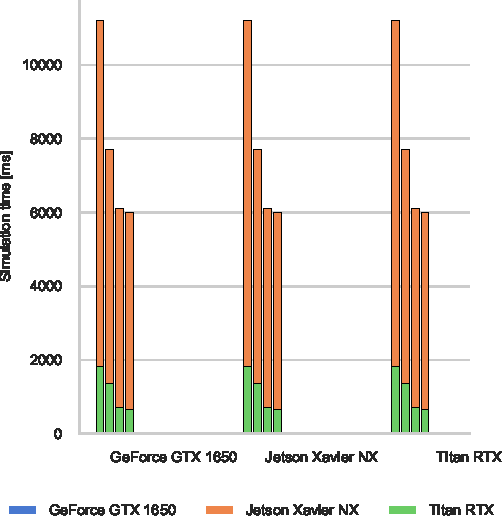
\includegraphics{figures/microcircuit_overheads.pdf}
    \end{center}
    \caption{Simulation times of the microcircuit model running on various GPU hardware for \SI{1}{\second} of biological time.
    `Overhead' refers to time spent in simulation loop but not within CUDA kernels.
    The dashed horizontal line indicates realtime performance}
    \label{fig:microcircuit_overheads}
\end{figure}
%
\begin{figure}[t!]
    \begin{center}
        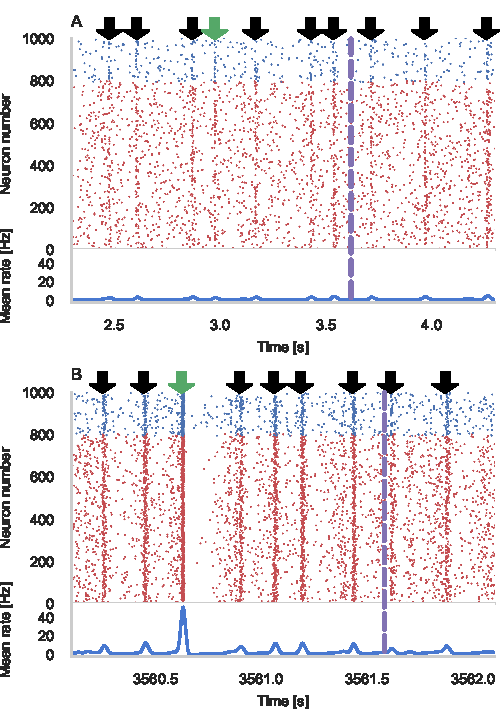
\includegraphics{figures/izhikevich_spikes.pdf}
    \end{center}
    \caption{Results of Pavlovian conditioning experiment.
             Raster and spike density plots showing activity centred around first delivery of Conditional Stimulus~(CS) during initial~(A) and final~(B) \SI{50}{\second} of simulation.
             Downward green arrows indicate times at which CS is delivered and downward black arrows indicate times when other, un-rewarded stimuli are delivered. 
             Vertical dashed lines indicate times at which dopamine is delivered}
    \label{fig:izhikevich_spikes}
\end{figure}
%
\section{Results}
In the following subsections we will analyse the performance of the models introduced in sections~\ref{sec:methods/cortical_microcircuit}~and~\ref{sec:methods/izhikevich} on a representative selection of NVIDIA GPU hardware:
%
\begin{itemize}
    \item Jetson Xavier NX -- a low-power embedded system with a GPU based on the Volta architecture with \SI{8}{\giga\byte} of shared memory.
    \item GeForce GTX 1050Ti -- a low-end desktop GPU based on the Pascal architecture with \SI{4}{\giga\byte} of dedicated memory.
    \item GeForce GTX 1650 -- a low-end desktop GPU based on the Turing architecture with \SI{4}{\giga\byte} of dedicated memory.
    \item Titan RTX -- a high-end workstation GPU based on the Turing architecture with \SI{24}{\giga\byte} of dedicated memory.
\end{itemize}
%
All of these systems run Ubuntu 18 apart from the system with the GeForce 1050 Ti which runs Windows 10.

\subsection{Cortical microcircuit model performance}
Figure~\ref{fig:microcircuit_overheads} shows the simulation times for the full-scale microcircuit model and, as one might predict, the Jetson Xavier NX is slower than the three desktop GPUs.
However, considering that it only consumes a maximum of \SI{15}{\watt} compared to \SI{75}{\watt} or \SI{320}{\watt} for the GeForce cards and Titan RTX respectively, it still performs impressively.
The time taken to actually simulate the models (`Neuron simulation' and `Synapse simulation') are the same when using Python and C++ as all GeNN optimisation options are exposed to PyGeNN.
Interestingly, when simulating \emph{this} model, the larger L1 cache and architectural improvements present in the Turing-based GTX 1650 do not result in significantly improved performance over the Pascal-based GTX 1050Ti.
Instead, the slightly improved performance of the GTX 1650 can probably be explained by its additional \num{128} CUDA cores.

Without the recording system described in section~\ref{sec:methods/spike_recording}, the CPU and GPU need to to synchronised after every timestep to allow spike data to be copied off the GPU and stored in a suitable data structure.
The `overheads' shown in figure~\ref{fig:microcircuit_overheads} indicate the time taken by these processes as well as the unavoidable overheads of launching CUDA kernels etc.
Because Python is an interpreted language, updating the spike data structures is somewhat slower and this is particularly noticeable on devices with a slower CPU such as the Jetson Xavier NX.
However, unlike the desktop GPUs, the Jetson Xavier NX's \SI{8}{\giga\byte} of memory is shared between the GPU and the CPU meaning that data doesn't have to be copied between their memories and can instead by accessed by both.
While, using this shared memory for recording spikes reduces the overhead of copying data off the device, because the GPU and CPU caches are not coherent, caching must be disabled on this memory which reduces the performance of the neuron kernel.
Although the Windows machine has a relatively powerful CPU, the overheads measured in both the Python and C++ simulations run on this system are extremely large due to additional queuing between the application and the GPU driver  caused by the Windows Display Driver Model~(WDDM).
When small -- in this case \SI{0.1}{\milli\second} -- simulation timesteps are used, this makes per-timestep synchronisation disproportionately expensive.

However, when the spike recording system described in section~\ref{sec:methods/spike_recording} is used, spike data is kept in GPU memory until the end of the simulation and overheads are reduced by up to 10$\times$.
Because synchronisation with the CPU is no longer required every timestep, simulations run approximately twice as fast on the Windows machine.
%Intriguingly, the overhead is now identical between Python and C++.
Furthermore, on the high-end desktop GPU, the simulation now runs faster than real-time in both Python and native C++ versions -- significantly faster than other recently published GPU simulators~\citep{Golosio2020} and even specialised neuromorphic systems~\citep{Rhodes2019}.
%
\begin{figure}[t!]
    \begin{center}
        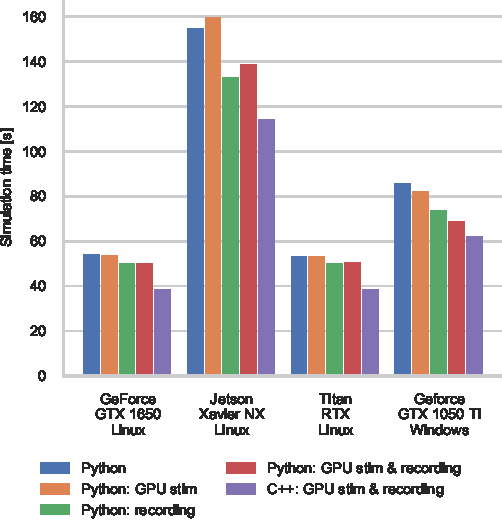
\includegraphics{figures/izhikevich.pdf}
    \end{center}
    \caption{Simulation times of the Pavlovian Conditioning model running on various GPU hardware for \SI{1}{\hour} of biological time.
             \todo{explanation of bars}}
    \label{fig:izhikevich}
\end{figure}
%
\subsection{Pavlovian conditioning performance}
Figure~\ref{fig:izhikevich_spikes} shows the results of an example simulation of the Pavlovian conditioning model.
At the beginning of each simulation (Figure~\ref{fig:izhikevich_spikes}A), the neurons representing every stimulus respond equally.
However, after \SI{1}{\hour} of simulation, the response to the CS becomes much stronger (Figure~\ref{fig:izhikevich_spikes}B) -- showing that these neurons have been selectively associated with the stimulus even in the presence of the distractors and the delayed reward.
%
\begin{figure}[t!]
    \begin{center}
        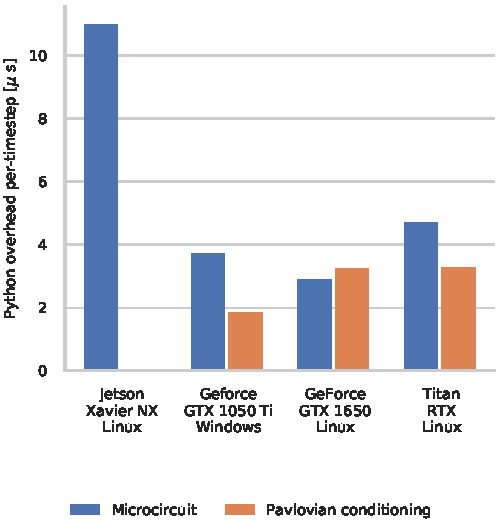
\includegraphics{figures/compare_overhead.pdf}
    \end{center}
    \caption{Comparison of per-timestep overhead in microcircuit and Pavlovian conditioning experiments.}
    \label{fig:compare_overhead}
\end{figure}

In figure~\ref{fig:izhikevich}, we show the runtime performance of simulations of the Pavlovian conditioning model, running on a selection of desktop GPUs using PyGeNN with and without the recording system described in section~\ref{sec:methods/spike_recording} and the optimized stimuli-delivery described in section~\ref{sec:methods/izhikevich}.
These PyGeNN results are compared to a C++ simulation using both optimizations.
Interestingly the Titan RTX and GTX 1650 perform identically in this benchmark with speedups ranging from $62\times$ to $72\times$ real-time.
This is because, as discussed previously, this model is simply not large enough to fill the \num{4608} CUDA cores present on the Titan RTX.
Therefore, as the two GPUs share the same Turing architecture and have very similar clock speeds (\SIrange{1350}{1770}{\mega\hertz} for the Titan RTX and \SIrange{1485}{1665}{\mega\hertz} for the GTX 1650), the two GPUs perform very similarly.
Furthermore, on these two systems, while using the recording system significantly improves performance, the impact of delivering stimuli on the GPU is minimal.
However, unlike in the simulations of the microcircuit model, here the GTX 1050 Ti performs rather differently. 
Although the clock speed of this device is approximately the same as the other GPUs (\SIrange{1290}{1392}{\mega\hertz}) and it has a similar number of CUDA cores to the GTX 1650, its performance is significantly worse.
The difference in performance across all configurations is likely to be due to architectural differences between the older Pascal; and newer Volta and Turing architectures.
Specifically, Pascal GPUs have one type of Arithmetic Logic Unit~(ALU) which handles both integer and floating point arithmetic whereas, the newer Volta and Turing architectures have equal numbers of dedicated integer and floating point ALUs as well as significantly larger L1 caches.
As discussed in our previous work~\citep{Knight2018}, these architectural features are particularly beneficial for SNN simulations with STDP where a large amount of floating point computation is required to update the synaptic state \emph{and} additional integer arithmetic is required to calculate the indices into the sparse matrix data structures.
Furthermore, due to the additional synchronisation overheads caused by the Windows Display Driver Model~(WDDM) which we discussed in the previous section, offloading stimuli delivery to the GPU improves the performance significantly on the Windows machine.

The difference between the speeds of the Python and C++ simulations of the Pavlovian conditioning model~(figure~\ref{fig:izhikevich}) \emph{appear} much larger than those of the microcircuit model~(figure~\ref{fig:microcircuit_overheads}).
However, as figure~\ref{fig:compare_overhead} illustrates, the difference between the duration of individual timestep in Python and C++ simulations of both models is approximately constant and consistent with the cost of a small number of Python to C++ function calls~\citep{Crail2019}.
However, depending on the size and complexity of the model as well as the hardware used, this overhead may still be significant.\todo{not really sure whether significant is what we want to say here}
For example, when simulating the microcircuit model for \SI{1}{\second} on the Titan RTX, the overhead of using Python is less than \SI{0.2}{\percent} but, when simulating the Pavlovian conditioning model on the same device, the overhead of using Python is almost \SI{31}{\percent}.

\section{Discussion}
In this paper we have introduced PyGeNN, a Python interface to the C++ based GeNN library for GPU accelerated spiking neural network simulations.

Uniquely, the new interface provides access to all the features of GeNN, without leaving the comparative simplicity of Python and with, as we have shown, typically negligible overheads from the Python bindings.
PyGeNN also allows bespoke neuron and synapse models to be defined from within Python, making PyGeNN much more flexible and broadly applicable than, for instance, the Python interface to NEST~\citep{Eppler2009} or the PyNN model description language used to expose CARLsim to Python~\citep{Balaji2020}.

In many ways, the new interface resembles elements of the Python-based Brian 2 simulator~\citep{Stimberg2019}~(and it's Brian2GeNN backend~\citep{Stimberg2020}) with two key differences.
Unlike in Brian 2, bespoke models in PyGeNN are defined with `C-like' code snippets. 
This has the advantage of unparalleled flexibility for the expert user but, comes at the cost of more complexity as the code for a timestep update needs to include a suitable solver as well as merely differential equations.
The second difference lies in how data structures are handled. 
Whereas simulations run using the C++ or Brian2GeNN Brian 2 backends use files to exchange data with Python, the underlying GeNN data structures are directly accessible from PyGeNN meaning that no disk access is involved.

As we have demonstrated, the PyGeNN wrapper, exactly like native GeNN, can be used on a variety of hardware from data centre scale down to mobile devices such as the NVIDIA Jetson.
This allows for the same codes to be used in large-scale brain simulations and embedded and embodied spiking neural network research.
Supporting the popular Python language in this interface makes this ecosystem available to a wider audience of researchers in both Computational Neuroscience, bio-mimetic machine learning and autonomous robotics.

The new interface also opens up opportunities to support researchers that work with other Python based systems.
In the Computational Neuroscience and Neuromorphic computing communities, we can now build a PyNN~\citep{Davison2008} interface on top of PyGeNN and, infact, a prototype of such an interface is in development.
Furthermore, for the burgeoning spike-based machine learning community, we can use PyGeNN as the basis for a spike-based machine learning framework akin to TensorFlow or PyTorch for rate-based models.
A prototype interface of this sort called mlGeNN is in development and close to release.

Finally, in this work we have introduced a new spike recording system for GeNN and have shown that, using this system, we can now simulate the Potjans microcircuit~\citep{Potjans2012} model faster than real-time, which thus far was only possible on the large SpiNNaker neuromorphic supercomputer~\citep{Rhodes2019}.

\begin{itemize}
  \item do we need to discuss the wide variety of uses, i.e. MC versus Pavlovian demonstrated in this paper?
    \item Turing architecture is great for GeNN! Presented results improve on state-of-the-art.
    \item PyGeNN as an intermediate layer - PyNN, ML
    \item Cost of C++ - Python calls in models
    \item something about neuromorphic systems often being real-time / BS accelerated time
\end{itemize}

\section*{Conflict of Interest Statement}
The authors declare that the research was conducted in the absence of any commercial or financial relationships that could be construed as a potential conflict of interest.

\section*{Author Contributions}
JK and TN wrote the paper.
TN is the original developer of GeNN.
AK was the original developer of PyGeNN.
JK is currently the primary developer of both GeNN and PyGeNN and was responsible for implementing the spike recording system.
JK performed the experiments and the analysis of the results that are presented in this work.

\section*{Funding}
This work was funded by the EPSRC (Brains on Board project, grant number EP/P006094/1).

\section*{Acknowledgments}
This is a short text to acknowledge the contributions of specific colleagues, institutions, or agencies that aided the efforts of the authors.

\section*{Data Availability Statement}
The datasets [GENERATED/ANALYZED] for this study can be found in the [NAME OF REPOSITORY] [LINK].
% Please see the availability of data guidelines for more information, at https://www.frontiersin.org/about/author-guidelines#AvailabilityofData

\bibliographystyle{frontiersinSCNS_ENG_HUMS} % for Science, Engineering and Humanities and Social Sciences articles, for Humanities and Social Sciences articles please include page numbers in the in-text citations
\bibliography{pygenn}

\end{document}
